\documentclass{article}

\usepackage{fullpage}
\usepackage{graphicx}

\title{Identification of the open loop dynamics of a bicycle-rider system
under manual control}
\author{Jason K. Moore}
\date{\today}

\begin{document}

\maketitle

Models that accurately predict the open loop behavior of a vehicle give
engineers a platform for analytical manipulation that can lead to desirable
open or closed loop dynamics. The bicycle is such a system but is unique when
compared more common vehicles such as automobiles and aircraft in that the
vehicle is almost always coupled with to a human who affects the systems
trajectory with both intended and unintended actions through a variety of body
motions. A model of the the open loop behavior of the bicycle-rider system is
critical for understanding the system.

Traditionally, mechanisists develop models of the bicycle-rider system from
first principles, i.e. Newton's laws and various other atomic fundamental
models of nature. The first principle approach has guided much of engineering
throughout its history but today's experiments are capable of delivering a
staggering amount of both kinematic and kinetic data for dynamicists. The
Whipple model \cite{Whipple1899} is often and highly regarded as a predictive
model of the bicycle-rider system and is constructed from first principles, yet
very little experimental data proves that the Whipple model is in fact a robust
model for the open loop dyamics of the bicycle-rider system. Motorcycle
researchers have long ago moved to more complex first principles models for
accurate prediction of the dynamics \cite{Sharp1971} and it is often questioned
why bicycle dynamicists continue to use the Whipple model for studies which are
more than purely academic in nature.

There is one attempt at experimentally validating the open-loop dynamics of the
bicycle-rider system for steady turns \cite{Cain2012} and only a handful that
attempt to identify a riderless bicycle
\cite{Kooijman2006,Kooijman2008,Kooijman2009,Stevens2009,Escalona2011,Kooijman2011}.
\cite{Cain2012} finds large descrepanices in predicted and measured steer
torque.  There are studies which identify the motorcycle-rider system but are
also of limited number and generally at much higher speeds than bicycles
travel.

Two remedy this, we have collected a large set of time history data which
includes the most important kinematic and kinetic variables to describe the
bicycle-rider motion (namely the roll and steer angles and rates, the applied
steer torque, and the wheel rate) from three different riders on the same
bicycle for a variety of manuevers and speeds. This generated about 1.7 million
time samples for each sensor collected at 200 hertz (representing about 2.4
hours) and has been made available online for easy reuse \cite{data}.

The instrumented bicycle was designed so that the riders were not able to move
their legs or torso relative to the rear frame of the bicycle, to ensure that
the assumption of rider rigidity of the Whipple bicycle model was as close to
valid as possible.

We start by simulating the Whipple model given carefully measured physical
parameters and the measured steer torque for each of the 374 runs and show that
the trajectories of the kinematic variables in the simulation are factor of
magnitude larger than the measurements of those same variables. We conclude
that the Whipple model requires much less steer torque to drive it through the
same trajectory as our real bicycle-rider system. This suggests that there is a
discrepency in the gain in the model which maps the kinetic inputs to the
kinematic outputs.

To rule out the possible invalidations of rigid rider assumptions due to us
allowing the rider to move his arms while controlling the bicycle we then
simulate a bicycle-rider model with the inertial effects of the rider's arms
(no extra degrees of freedom where added) in the same fashion as previously
described. The model with the arms shows better agreement to the measured data
than the Whipple model.

Finally, we make use of two system identification techniques to identify the
coefficients of the Whipple model in both state space form and
mass-spring-damper form. These identification methods result in various 4th
order models that predict the measured data accurately. When comparing the
Whipple model coefficients derived from first principles to the coefficients of
the identified models we find that the identified models do not generate
realistic values for the physical constants.

\begin{figure}
  \centering
  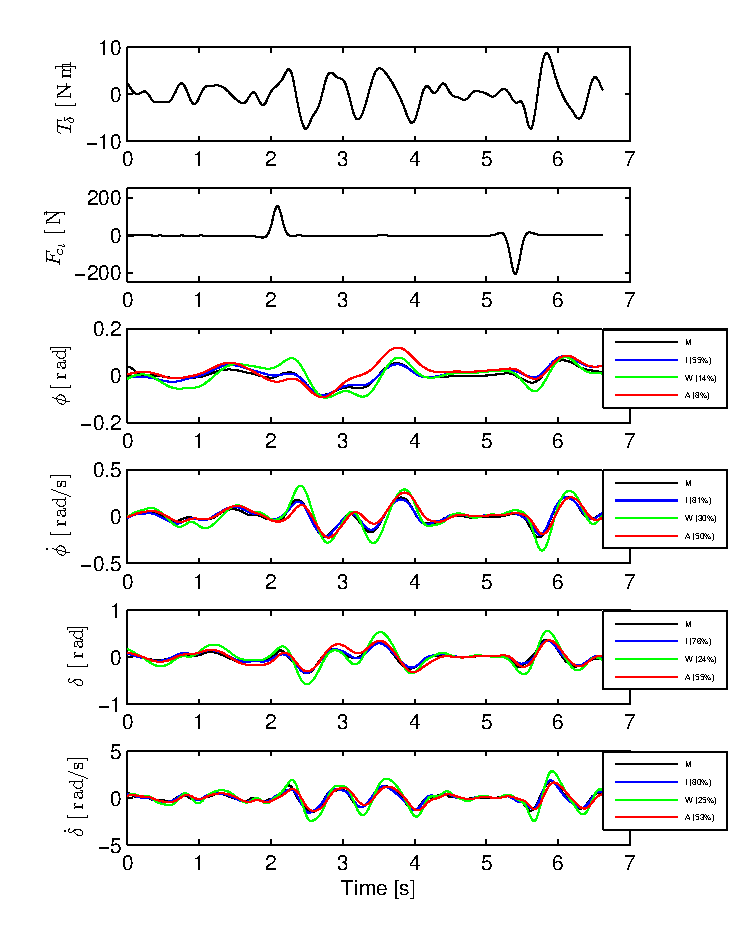
\includegraphics[width=5.0in]{example-fit.pdf}
  \caption{Example results for the identification of a single run (\#596). The
  experimentally measured steer torque and lateral force are shown in the top
  two graphs. All of the signals were filtered with a 2nd order 15 hertz low
  pass Butterworth filter. The remaining four graphs show the simulation
  results for the Whipple model (W), Whipple model with the arm inertia (A),
  and the identified model for that run (I) plotted with the measured data (M).
  The percentages give the percent of variance explained by each model.}
\end{figure}

In this paper we will show that a fourth order structured state space model is
both adequate for describing the motion of the bicycle under manual control in
a speed range from approximately 1.5 m/s to 9 m/s. The fact that higher order
models may not be necessary for bicycle dynamic description is an important
finding. More robust models of single track vehicles are typically higher than
4th order, with degrees of freedom associated with tire slip, frame
flexibilities, and rider biomechanics. These findings suggest that the more
complex models may be overkill for many modeling purposes.

The data subsequently also reveals that fourth order archetypal first
principles models, such as the Whipple model, are not robust enough to fully
describe the dynamics. The inability to identifying realisticallh valued
parameters points to model deficienes. The deficiencies are most likely due to
un-modeled effects, with the knife-edge, no side-slip wheel contact assumptions
being the most probable candidate. Un-modeled rider biomechanics such as
passive arm stiffness and damping and head motion may play a role too.

This paper is based on work supported by the National Science Foundation under
Grant No 0928339.

\bibliographystyle{plain}
\bibliography{bicycle}

\end{document}
